\documentclass[utf8,compress]{beamer}
\usepackage{irbookslide}
\usepackage{irilmenau2}
\usepackage{url}
\usepackage{fontspec} % zahteva paket euenc
\usepackage{xunicode}
\usepackage{xltxtra}
\usepackage{polyglossia}
\usepackage{minted}
\usepackage{xcolor,colortbl}
\usepackage{textcomp}
\usepackage{unicode-math}

\title{GUI aplikacije i PyQt}
\subtitle{\tiny{Slajdovi za predmet Osnove programiranja}}
\subject{Osnove programiranja}
\institute{Katedra za informatiku, Fakultet tehničkih nauka, Novi Sad}
\date{2014.}

\begin{document}
% da pygmentize ne uokviruje crvenom bojom nepoznate karaktere
\expandafter\def\csname PY@tok@err\endcsname{}

\frame{\titlepage}

\frame{
  \frametitle{Ciljevi}
  \begin{itemize}
    \item GUI = graphical user interface
    \item savlađivanje osnovnih koncepata pisanja GUI aplikacija
  \end{itemize}
}

\section[PyQt]{PyQt}

\begin{frame}[fragile]
  \frametitle{GUI biblioteke i Python}
  \begin{itemize}
    \item pisanje programa koji ima GUI od nule je ogroman posao
    \item puno istih funkcija bismo morali da pišemo iznova za svaki program
    \item $\Rightarrow$ možemo da koristimo \myblue{biblioteku klasa}
    \item za Python ih ima mnogo:
    \begin{itemize}
      \item TkInter
      \item wxPython
      \item PyQt
      \item PyGTK
      \item ...
    \end{itemize}
  \end{itemize}
\end{frame}

\begin{frame}[fragile]
  \frametitle{PyQt}
  \begin{itemize}
    \item Qt je cross-platform biblioteka za C++
    \begin{itemize}
      \item Windows, Linux, Mac OSX, Symbian, Android, iOS
    \end{itemize}
    \item PyQt je Python omotač oko Qt biblioteke
  \end{itemize}
\end{frame}

\begin{frame}[fragile]
  \frametitle{Struktura GUI aplikacije}
  \begin{itemize}
    \item bez obzira na izabranu GUI biblioteku, svaki program ima sličnu strukturu
    \item program se ne izvršava linearno (od početka prema kraju, bez pauze), već se izvršava samo u pojedinim trenucima \\ \ \\
    \item[1] inicijalizacija programa prilikom pokretanja 
    \begin{itemize}
      \item inicijalizuju se interne strukture podataka
    \end{itemize}
    \item[2] prepuštanje kontrole OS-u i čekanje na događaje
    \begin{itemize}
      \item mouse click, key press, touch, swipe, ...
    \end{itemize}
    \item[3] obrada nastalog događaja i prelazak na \myblue{2}
  \end{itemize}
\end{frame}

\begin{frame}[fragile]
  \frametitle{Prva GUI aplikacija}
\begin{minted}{python}
import sys
from PyQt4 import QtGui

def main():    
    app = QtGui.QApplication(sys.argv)
    w = QtGui.QWidget()
    w.resize(250, 150)
    w.move(300, 300)
    w.setWindowTitle('Prvi GUI program')
    w.show()
    # ovde je petlja za obradu događaja
    sys.exit(app.exec_())

if __name__ == '__main__':
    main()
\end{minted}
\end{frame}

\begin{frame}[fragile]
  \frametitle{Struktura GUI aplikacije}
  \begin{itemize}
    \item prozor već ima dosta funkcionalnosti (close, resize)
    \item nismo morali da pišemo sve od početka
  \end{itemize}
  \begin{center}
    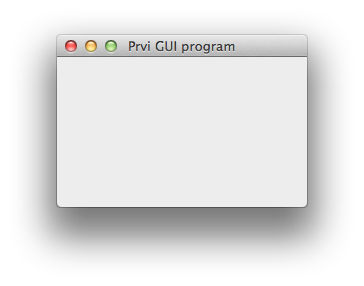
\includegraphics[width=8cm]{pyqt01.png}
  \end{center}
\end{frame}

\end{document}